\documentclass[a4paper,10pt]{article}
\usepackage[utf8]{inputenc}
\usepackage{graphicx}
\usepackage{framed} 
\usepackage{xcolor}
\usepackage{tcolorbox}
\usepackage{xcolor} 
\usepackage{framed} 
\usepackage{xcolor}
\usepackage{tcolorbox}
\usepackage{xcolor} 
\colorlet{shadecolor}{gray!25}
%opening
\title{Lab-report 5}
\author{Moritz Rupp}

\begin{document}
\maketitle
\tableofcontents
\begin{abstract}
Lab 5 Dokumentation
\end{abstract}
\newpage
\section{Exercise 5.1 - Basic repeated XOR encryption}
We are provided with a small python programm and a .txt file that includes the encrypted flag. The programm is a self made crypto implementation that should be easy to crack.\\
After analysing the code we realize that the key lenght is only 4 characters long.	
\begin{center}
 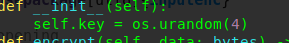
\includegraphics[scale=0.5]{keylen.png}
\end{center}
Thanks to the provided hint we also see the we are given the first 4 characters of the encrypted stream, since the HTB flags always follow the same format. This matches the key lenght.
\begin{center}
 \begin{shaded}
 HTB\{SOME\_FLAG\}\\
 $\Rightarrow$ HTB\{ 
\end{shaded}
\end{center}
We also know that xor operations are beeing performed. Hence we take the ASCII values of the known plaintext characters and xor them with the first 4 characters of the encrypted stream.
\begin{center}
4854427b xor 134af6e1\\
$\Rightarrow$ 5b1eb49a
\end{center}
This should be the key to decrypt the whole sequence. With the help of an online tool we get the correct key.
\begin{center}
 \begin{shaded}
 HTB\{rep34t3d\_x0r\_n0t\_s0\_s3cur3\}
 \end{shaded}
\end{center}
\newpage
\subsection{Exercise 5.2 - AES-CBC Decryption Oracle}




\end{document}
